\documentclass[main]{subfiles}

\begin{document}
  \begin{lect}{2019-09-09 Дифф. геометрия кривых (в $\R^3$) и поверхностей (в $\R^3$)}
    \section{Дифференциальная геометрия кривых}
    \subsection{Векторнозначная функция, её производная. Свойства.}
    \begin{definition}
        $f:[a,b] \rightarrow \R^3$ - вектор-функция. Образ f называется кривой, а f - параметризация этой кривой.
    \end{definition}

    Способы задания кривых:
    \begin{enumerate}
        \item Параметрический $f:[a,b] \rightarrow \R^3$
        \item Явное задание кривой $\begin{cases} y=y(x)\\ z=z(x)
        \end{cases}$

        (особенно хорошо на плоскости $y=f(x)$)
        \item Неявное задание кривой (на плоскости) $F(x,y)=0$
        \begin{Example}
            \[\text{Окружность: } x^2 + y^2 - 1 = 0\]
            \[y = \pm \sqrt{1 - x^2} \text{ явное задание}\]
            \begin{figure}[H]
                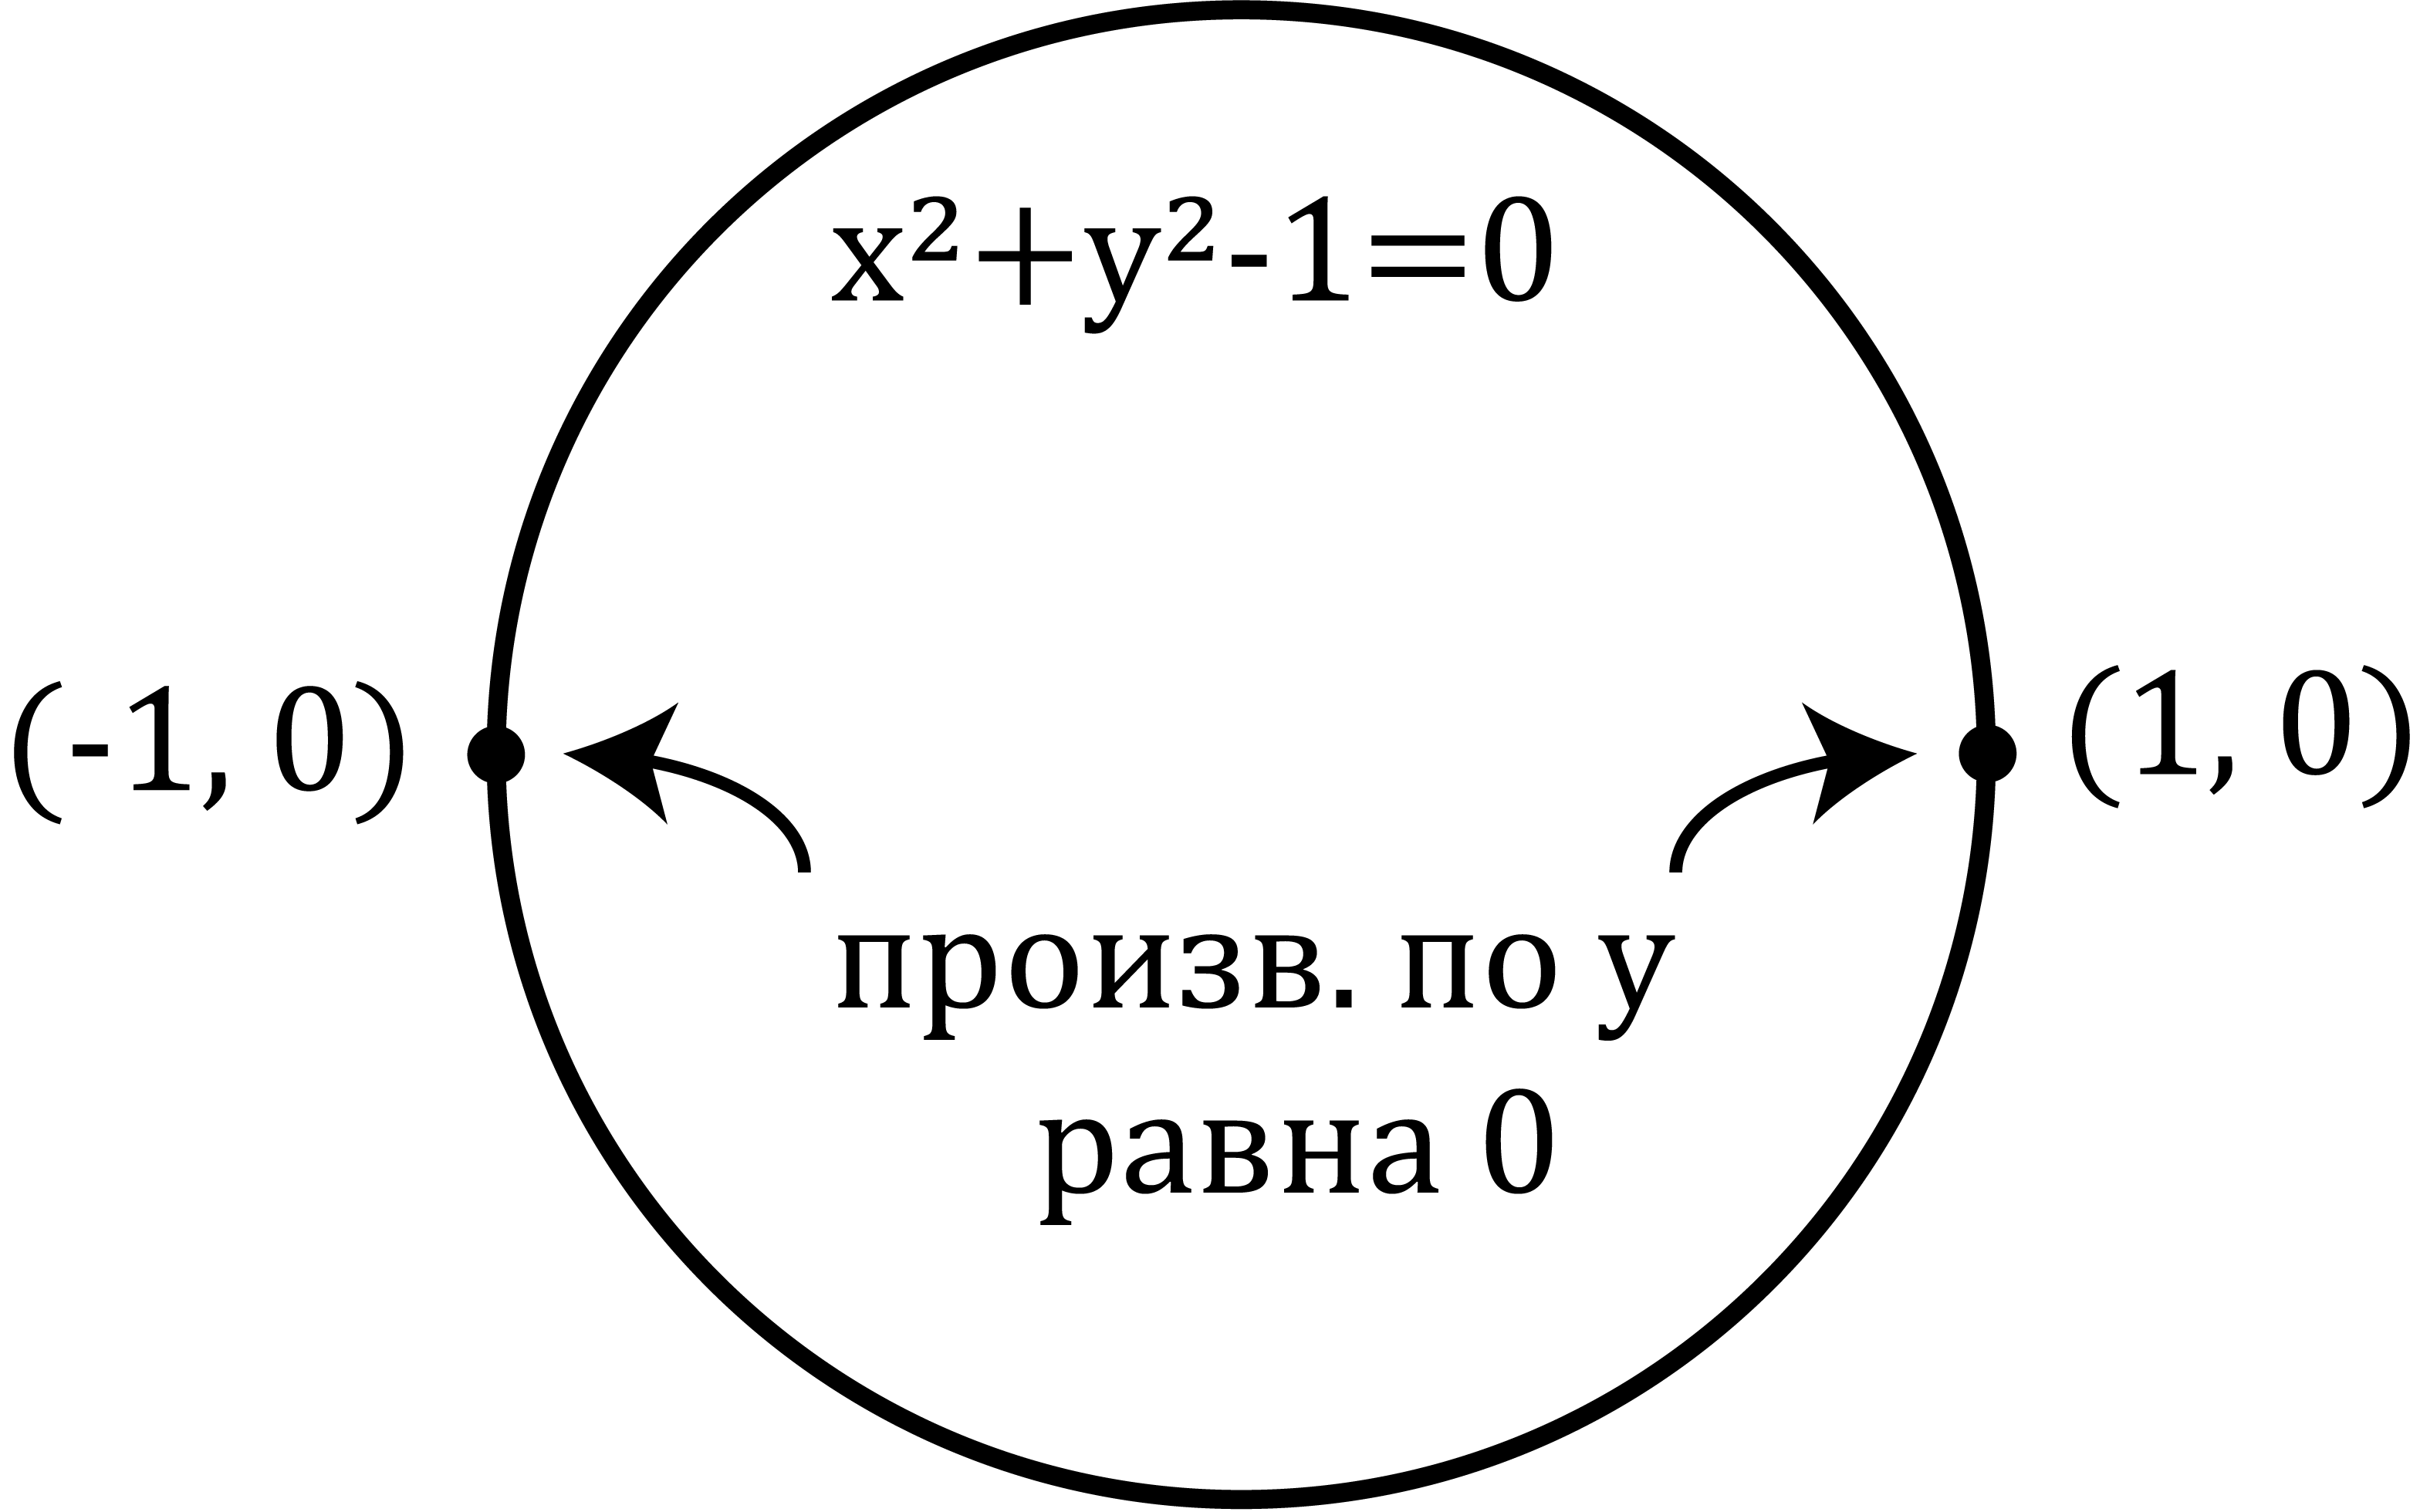
\includegraphics[width=5cm]{pics/1_1}
                \centering
            \end{figure}
        \end{Example}
    \end{enumerate}

    \begin{Theorem} [о неявной функции]
    	\[F(x, y) = 0\]
    	\[F \text{ - дифф } (\exists \frac{\partial F}{ \partial x} \text{ и }
    	\frac{\partial F}{\partial y} \text{ - непр в окр } (x_0, y_0)),\q F(x_0, y_0) = 0\]
    	\[\text{Если } \frac{\partial F}{\partial y} (x_0, y_0)  \neq  0 \Ra
    		\ \exists \mathcal{E} > 0 \ \exists f:
    	(x_0 - \mathcal{E}, x_0 + \mathcal{E}) \to \R\]
    	\[F(x, f(x)) = 0\]
    \end{Theorem}

    \begin{Reminder}
        \[\dfrac{dF}{dx} \Big |_{(x_0,y_0)}=\lim\limits_{x \rightarrow x_0} \frac{F(x,y_0)-F(x_0,y_0)}{x-x_0}\]
    \end{Reminder}

    \[y=f(x) \rightarrow \begin{cases} x=t\\ y=f(t) \end{cases}\q f(t)=(x(t),y(t),z(t))\]

    Как задавать вектор-функцию? $f:[a,b] \rightarrow \R^3$ - вектор-функция, тогда

    $\lim\limits_{t \rightarrow t_0} f(t) = (x_0, y_0, z_0)$
    \begin{multline*}
    	\forall \E > 0 \  \exists  \delta > 0: \text{ если } \rho (t,t_0) < \delta ,
        \text{ то } \rho(f(t),(x_0,y_0, z_0)) < \E \\
    	( \rho (t,t_0) = |t-t_0| , \q \sqrt{(x(t)-x_0)^2+(y(t)-y_0)^2+(z(t)-z_0)^2})
    \end{multline*}

    \begin{Theorem} [свойства пределов]
    	\[ \lim_{t \to t_0} (f(t) \pm g(t)) = \lim_{t \to t_0} f(t) \pm \lim_{t \to t_0} g(t)\]
    	\[ \lim_{t \to t_0} \underset{\text{скал}}{(f(t) \cdot g(t))} = (\lim_{t \to t_0} f(t) , \lim_{t \to t_0} g(t) )
    	\text{ - скалярное умножение}\]
    	\[ \lim_{t \to t_0} (f(x) \times g(t)) = \lim_{t \to t_0} f(x) \times \lim_{t \to t_0} g(t) \]
    \end{Theorem}

    \begin{Proof}
    	\[ \lim_{t \to t_0} f(t) = ( \lim_{t \to t_0} x(t), \lim_{t \to t_0} y(t), \lim_{t \to t_0} z(t))  )\]
    	\[f(t) = (x(t), y(t), z(t))\]
    	\[\text{Пусть } \E > 0, \q \text{выберем } \delta : |x(t) - x_0| < \frac{\mathcal{E}}{3}\]
    	\begin{multline*}
    		\text{если } |t - t_0| < \delta \\\Ra
    		\begin{align}
    			|y(t) - y_0| < \frac{\mathcal{E}}{3}\\
    			|z(t) - z_0| < \frac{\mathcal{E}}{3}
    		\end{align}
    		\Ra \sqrt{(x(t)-x_0)^2+(y(t)-y_0)^2+(z(t)-z_0)^2} < \frac{\E}{\sqrt{3}}
    	\end{multline*}
    \end{Proof}

    \begin{Definition}
    	\[f'(t_0) = \lim_{t \to t_0} \frac{ \overline{f}(t) - \overline{f}(t_0)}{t - t_0}\]
    \end{Definition}

    \begin{theorem} [свойства]
    		\begin{enumerate}
    			\item $(f(t) \pm g(t))' = f'(t) \pm y'(t)$
    			\item $(c f(t))' = cf'(t)$
    			\item $(f(t); g(t))' = (f'(t); g(t)) + (f(t); g'(t))$
    			\item $(f(t) \times g(t))' = f'(t) \times g(t) + f(t) \times g'(t)$
    			\item $(f(t), g(t), h(t))' = (f', g, h) + (f, g', h) + (f, g, h')$
    		\end{enumerate}

    		\[\text{Доказывается через }f'(t) = (x'(t), y'(t), z'(t))\]
    		\[f(t) = (x(t), y(t), z(t))\]

    		\[\text{Докажем ВП: }(f(t) \times g(t))'|_{t = t_0} = \lim_{t \to t_0} \frac{f(t) \times g(t) - f(t_0) \times g(t_0)}{t - t_0} = \]
    		\[= \lim_{t \to t_0} \frac{f(t) \times g(t) - f(t_0) \times g(t) + f(t_0) \times g(t) - f(t_0) \times g(t_0)}{t - t_0}\]
    		\[= \lim_{t \to t_0} \frac{(f(t) - f(t_0)) \times g(t)}{t - t_0} +
    		\lim_{t \to t_0} \frac{f(t_0) \times (g(t) - g(t_0))}{t - t_0} = \]
    		\[= f'(t_0) \times g(t_0) + f(t_0) \times g'(t_0)\]
    \end{theorem}

    \begin{example}
    		Контрпример\\
    		Т. Лагранжа  - неверна рис 4
    \end{example}

    \[\int_b^a \overrightarrow{f}(t) dt = (\int_a^b x(t)d(t), \int_a^b y(t)dt, \int_a^b z(t)dt) \]
    \[\overrightarrow{F}'(t) = \overrightarrow{f}(t)\]
    \[\overrightarrow{F}(b) - \overrightarrow{F}(a) = \int_a^b \overrightarrow{f}(t)dt\]
    \[F(t) = (X(t), Y(t), Z(t))\]
    \[f(t) = (X'(t), Y'(t), Z'(t)) = (x(t), y(t), z(t))\]
    \[\int_a^b f(t)dt = (\int_a^b x(t) dt, ....) = (X(b) - X(a), ....\]

    \begin{definition}
        Гладкая кривая - диффер. векторнозначная функция, ее образ тоже
    \end{definition}

    \begin{definition}
        Кривая называется регулярной, если существует производная и\\
    	$f'(t) \neq \overrightarrow{0}$
    \end{definition}

    \begin{definition}
        Кривая называется бирегулярной, если существует вторая производная и $f''(t) \not \parallel f'(t)$
    \end{definition}

    \begin{definition}
    	Параметризации $\overrightarrow{f}(t) $ и $\overrightarrow{g}(t)$ эквивалентны
    	\[f: [a, b] \to \R^3\]
    	\[g: [c, d] \to \R^3\]
    	Если $\exists$ биекция $\tau: [a, b] \to [c,d]$
    	\[\tau(a) = c; \q \tau(b) = d:\]
    	\[f(t) = g(\tau(t)) \q\q (\tau \text{ возрастает и гладкая})\]
    \end{definition}

    \begin{lemma}
    	Эквив параметризаций - эквививалентность
    \end{lemma}

    \begin{proof}
    	Докажем, что экв. параметризаций - отношение эквивалентности:
        \begin{enumerate}
            \item (рефл.) $\tau=id$
            \item (симм.) $f(t)=g(\tau(t))$, \q $g(t)=f(\tau(t))$
            \item (тран.) $f(t)=g(\sigma(t))$,\q $g(t)=h(\tau(t))$,\q $f(t)=h(\tau(\sigma(t)))$
        \end{enumerate}
    \end{proof}

    \begin{Lemma}
    	\[\overrightarrow{f}(t) \text{ - вектор-функция/ регуляр.}\]
    	\[|\overrightarrow{f}(t)| = 1 \Ra f'(t) \perp f(t)\]
    \end{Lemma}

    \begin{Proof}
    	\[(f(t); f(t)) = 1\]
    	\[0 = (f(t), f(t))' = 2(f'(t), f(t))\]
    	\[f(t) \neq 0\]
    	\[f'(t) \neq 0 \Ra f'(t) \perp f(t)\]
    \end{Proof}
  \end{lect}
\end{document}
